\chapter{Testowanie metod klastrowania}
\label{ch:testwy}
\section{Środowisko testowe}
Wszystkie rozwiązania testowane będą przy użyciu następującego środowiska testowego:
\begin{description}
\item{Maszyna fizyczna:}
    \begin{itemize}
	\item CPU: \texttt{Intel(R) Core(TM)2 Quad CPU    Q9400 @ 2.66GHz} posiadający wsparcie dla wirtualizacji (\textit{VT-x})
	\item Pamięć RAM: \texttt{8G DDR2}
%%	\item OS: \texttt{Linux redraptor 3.18.1-gentoo \#7 SMP Wed Dec 31 02:04:37 CET 2014 x86\_64}
	\item OS: \texttt{Gentoo Linux 64bit, kernel 3.18.1}
	\item Platforma wirtualizacyjna: \texttt{KVM} (host)
    \end{itemize}
\item{Maszyna wirtualna na potrzeby kontenerów:}
    \begin{itemize}
	\item CPU: Mapowany z maszyny fizycznej. Przydział 3 rdzeni
	\item Pamięć RAM: \texttt{2G}
%%	\item OS: \texttt{Linux lxc 3.13.0-24-generic \#46-Ubuntu SMP Thu Apr 10 19:11:08 UTC 2014 x86\_64 x86\_64 x86\_64}
	\item OS: \texttt{Ubuntu Linux 64 bit, kernel 3.13.0-24-generic}
	\item Platforma wirtualizacyjna: \texttt{KVM} (guest), \texttt{LXC} (host)
    \end{itemize}
\item{Kontenery \texttt{LXC} do celów testowania aplikacji:}
    \begin{itemize}
	\item OS: Ubuntu linux. Jądra współdzielone z maszyną hostującą.
	\item Ustawienia \texttt{cgroups}: \texttt{lxc.cgroup.cpu.cfs\_quota\_us = 30000}
    \end{itemize}
\item{Maszyna wirtualna na potrzeby \texttt{LVS}:}
    \begin{itemize}
	\item CPU: Mapowany z maszyny fizycznej. Przydział 1 rdzeń
%%    	\item OS: \texttt{Linux mgr10 3.13.0-24-generic \#46-Ubuntu SMP Thu Apr 10 19:11:08 UTC 2014 x86\_64 x86\_64 x86\_64}
	\item OS: \texttt{Ubuntu Linux 64 bit, kernel 3.13.0-24-generic}
	\item Pamięć RAM: \texttt{192M}
    \end{itemize}
\end{description}
Aplikacje działające w \texttt{userspace}, tj. \texttt{apache, nginx, haproxy, php-fpm}, zostają uruchamiane w dedykowanych kontenerach \texttt{LXC}.
Usługi działające w warstwie jądra, tj. \texttt{LVS} zostają uruchomione na dedykowanej maszynie wirtualnej przy użyciu \texttt{KVM}.
\section{Wybór serwera WWW}
\label{sec:wybor}
W rozdziale tym zostanie przedstawione zestawienie kilku testów wydajnościowych dwóch serwerów WWW\@.
\begin{itemize}
\item Apache2
\item Nginx
\end{itemize}
Przetestowane zostanie serwrowanie plików statycznych oraz treści dynamicznych PHP{.}\\
Wszystkie testy zostały przeprowadzone z wykorzystaniem 10 000 połączeń.\\
Wszystkie czasy zostały podane w milisekundach.
\subsection{Pliki statyczne}
Testy plików statycznych przeprowadzone zostaną przy użyciu dwóch plików HTML{.}
Jeden o rozmiarze 10 bajtów, drugi o rozmiarze 100 kilobajtów.

\begin{figure}
	\centering
	\begin{subfigure}[h]{0.3\textwidth}
		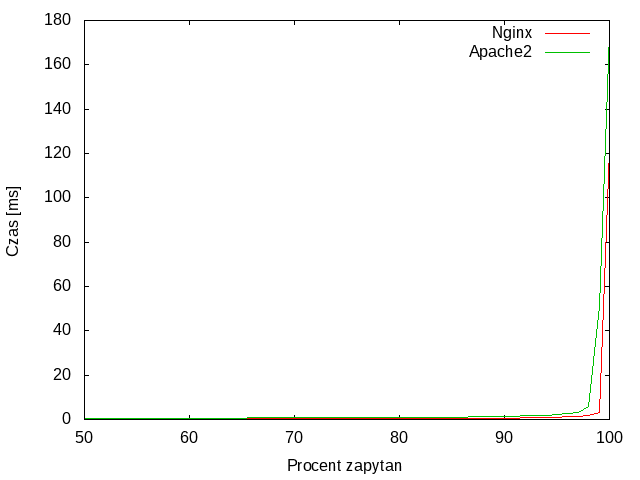
\includegraphics[width=\textwidth]{testy/wybor_index_maly_1.png}
		\caption{1 równoległe zapytanie}
	\end{subfigure}
	\begin{subfigure}[h]{0.3\textwidth}
		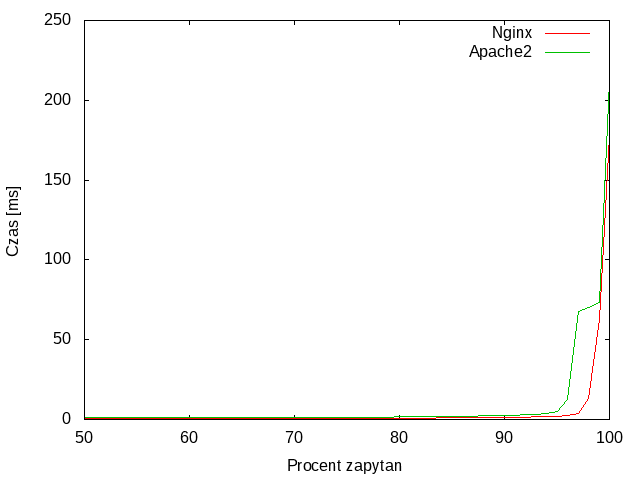
\includegraphics[width=\textwidth]{testy/wybor_index_maly_2.png}
		\caption{2 równoległe zapytania}
	\end{subfigure}
	\begin{subfigure}[h]{0.3\textwidth}
		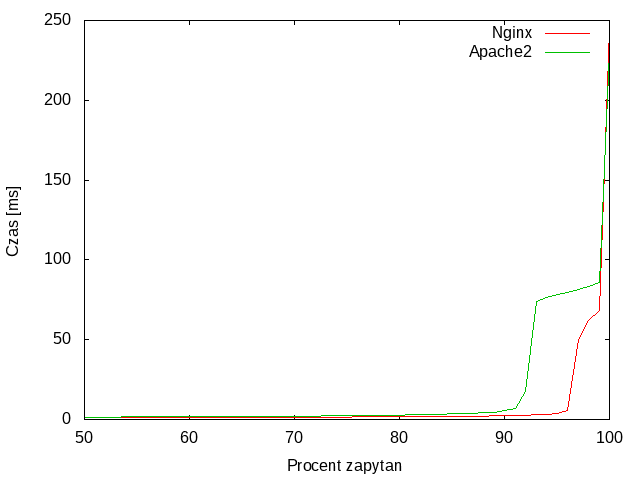
\includegraphics[width=\textwidth]{testy/wybor_index_maly_4.png}
		\caption{4 równoległe zapytania}
	\end{subfigure}

	\begin{subfigure}[h]{0.3\textwidth}
		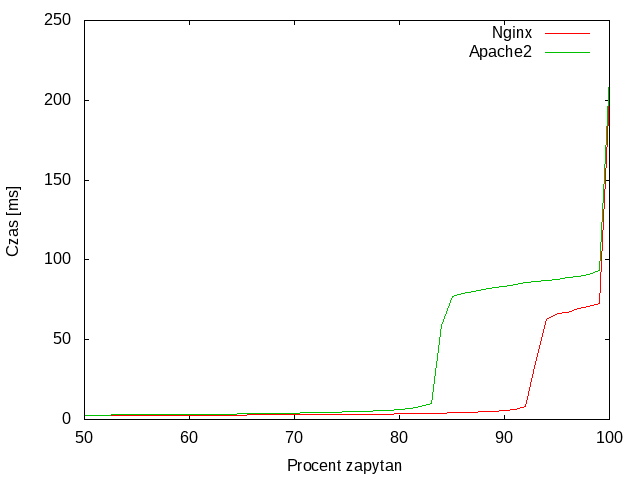
\includegraphics[width=\textwidth]{testy/wybor_index_maly_8.png}
		\caption{8 równoległych zapytań}
	\end{subfigure}
	\begin{subfigure}[h]{0.3\textwidth}
		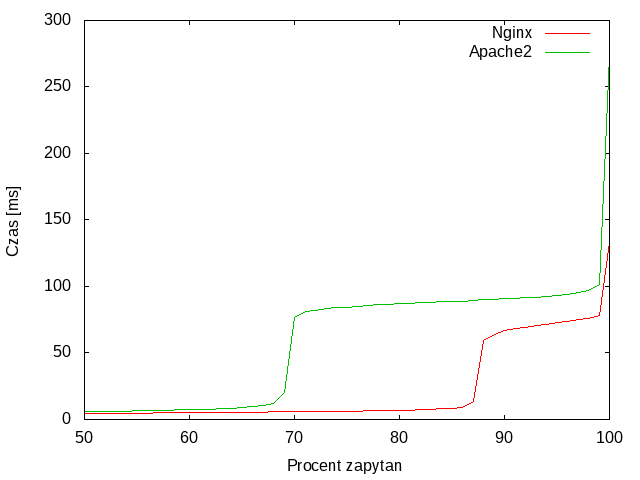
\includegraphics[width=\textwidth]{testy/wybor_index_maly_16.png}
		\caption{16 równoległych zapytań}
	\end{subfigure}
	\begin{subfigure}[h]{0.3\textwidth}
		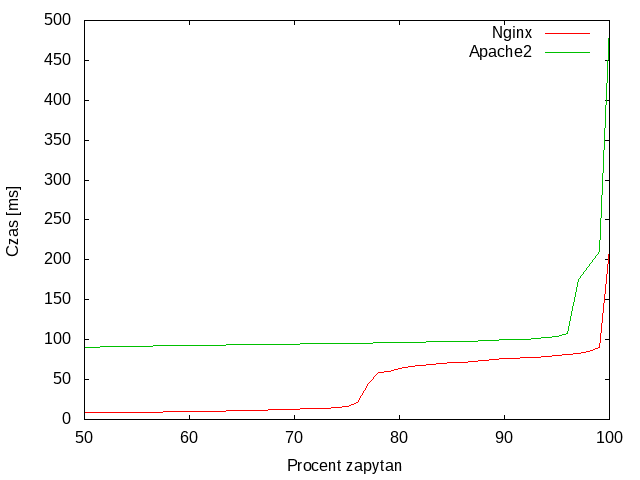
\includegraphics[width=\textwidth]{testy/wybor_index_maly_32.png}
		\caption{32 równoległe zapytania}
	\end{subfigure}

	\begin{subfigure}[h]{0.3\textwidth}
		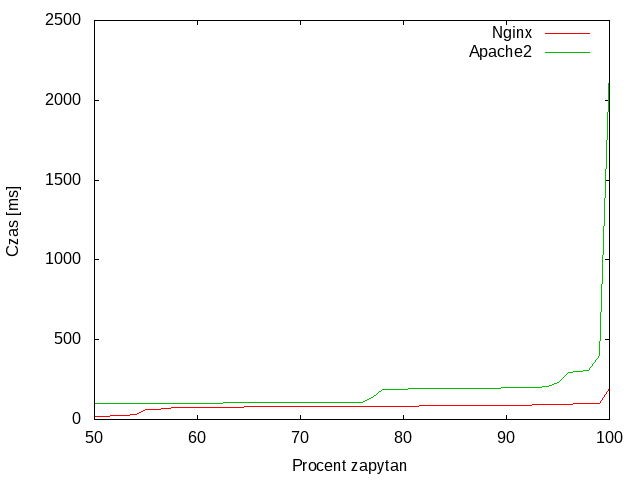
\includegraphics[width=\textwidth]{testy/wybor_index_maly_64.png}
		\caption{64 równoległe zapytania}
	\end{subfigure}
	\begin{subfigure}[h]{0.3\textwidth}
		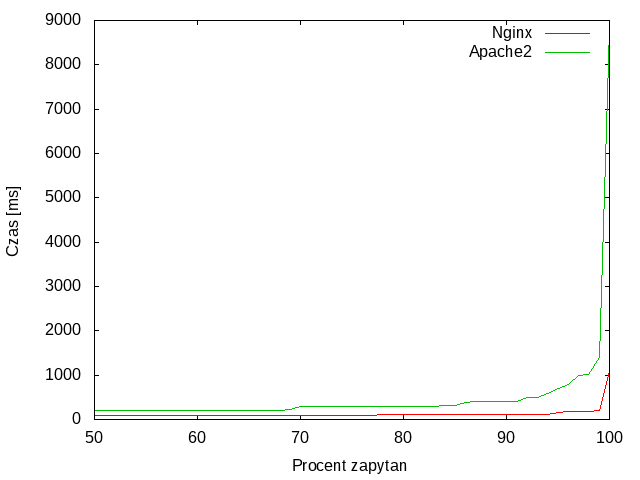
\includegraphics[width=\textwidth]{testy/wybor_index_maly_128.png}
		\caption{128 równoległe zapytania}
	\end{subfigure}
	\begin{subfigure}[h]{0.3\textwidth}
		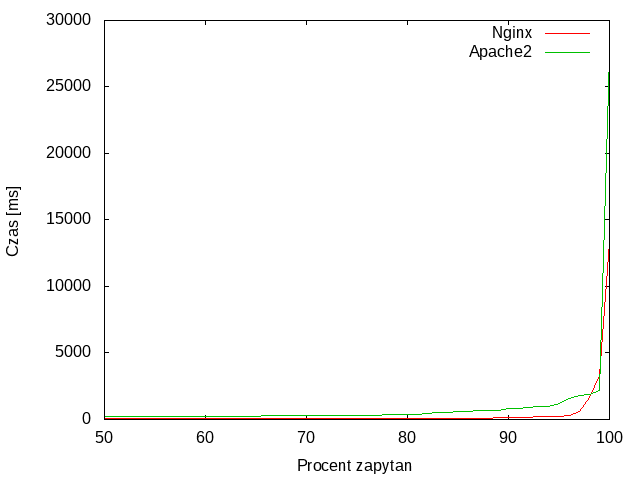
\includegraphics[width=\textwidth]{testy/wybor_index_maly_256.png}
		\caption{256 równoległych zapytań}
	\end{subfigure}
	\caption{Zapytania o mały plik statyczny}\label{fig:wyb_index_maly}
\end{figure}
\begin{figure}
	\centering
	\begin{subfigure}[h]{0.3\textwidth}
		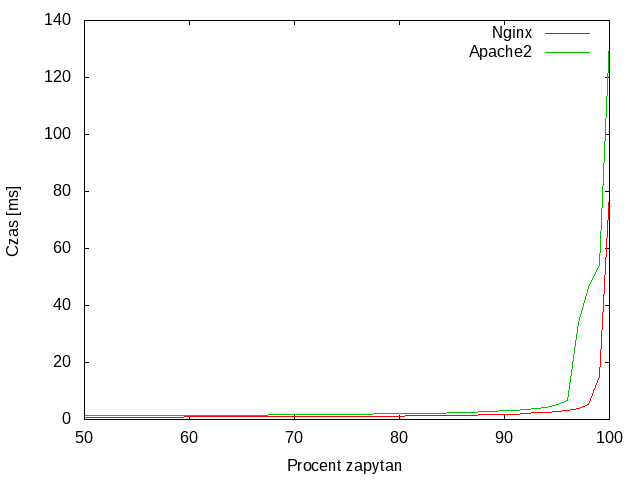
\includegraphics[width=\textwidth]{testy/wybor_index_duzy_1.png}
		\caption{1 równoległe zapytanie}
	\end{subfigure}
	\begin{subfigure}[h]{0.3\textwidth}
		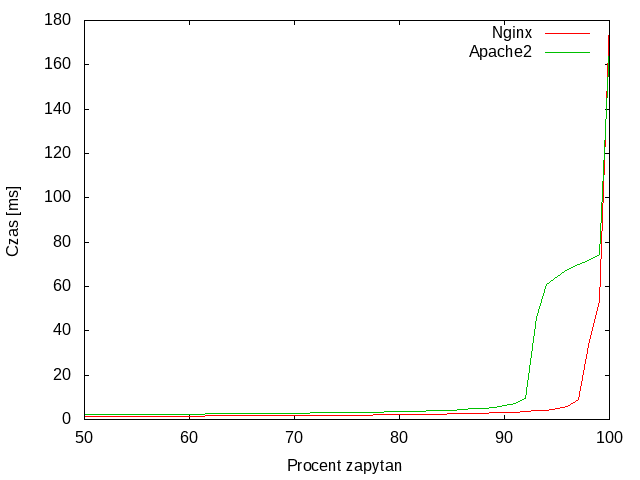
\includegraphics[width=\textwidth]{testy/wybor_index_duzy_2.png}
		\caption{2 równoległe zapytania}
	\end{subfigure}
	\begin{subfigure}[h]{0.3\textwidth}
		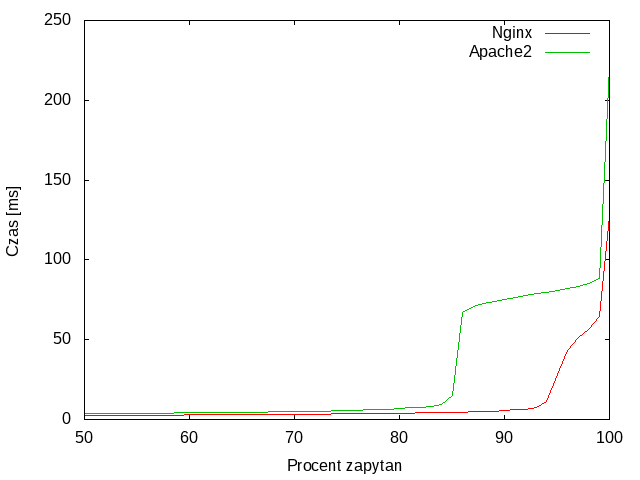
\includegraphics[width=\textwidth]{testy/wybor_index_duzy_4.png}
		\caption{4 równoległe zapytania}
	\end{subfigure}

	\begin{subfigure}[h]{0.3\textwidth}
		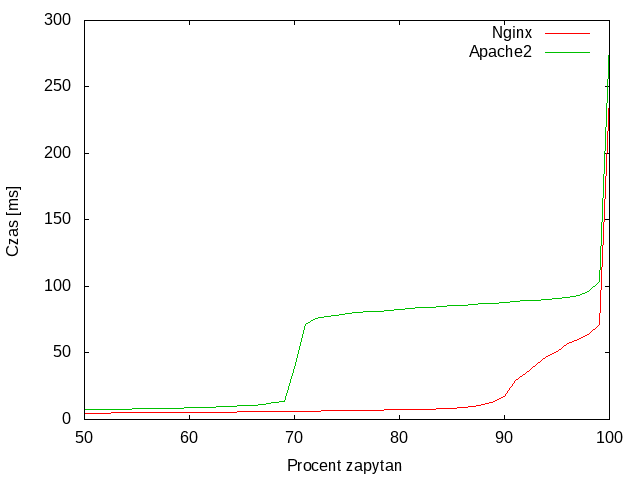
\includegraphics[width=\textwidth]{testy/wybor_index_duzy_8.png}
		\caption{8 równoległych zapytań}
	\end{subfigure}
	\begin{subfigure}[h]{0.3\textwidth}
		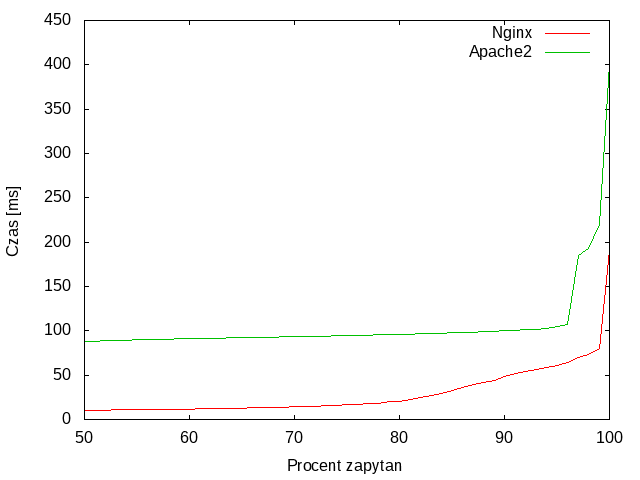
\includegraphics[width=\textwidth]{testy/wybor_index_duzy_16.png}
		\caption{16 równoległych zapytań}
	\end{subfigure}
	\begin{subfigure}[h]{0.3\textwidth}
		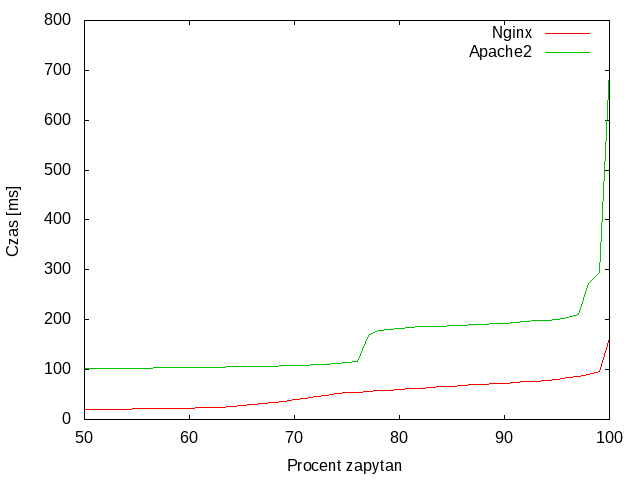
\includegraphics[width=\textwidth]{testy/wybor_index_duzy_32.png}
		\caption{32 równoległe zapytania}
	\end{subfigure}

	\begin{subfigure}[h]{0.3\textwidth}
		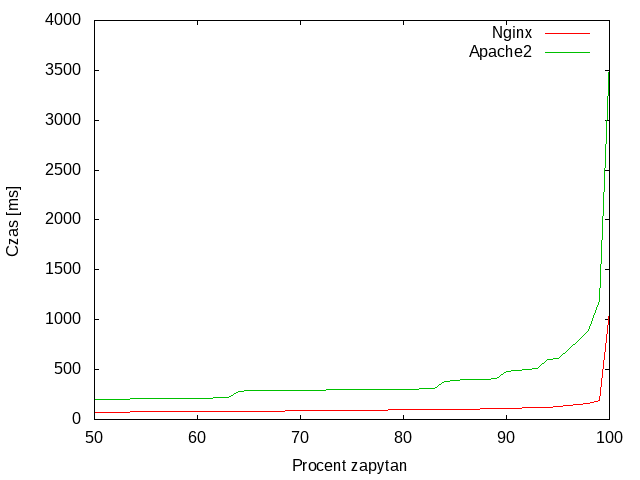
\includegraphics[width=\textwidth]{testy/wybor_index_duzy_64.png}
		\caption{64 równoległe zapytania}
	\end{subfigure}
	\begin{subfigure}[h]{0.3\textwidth}
		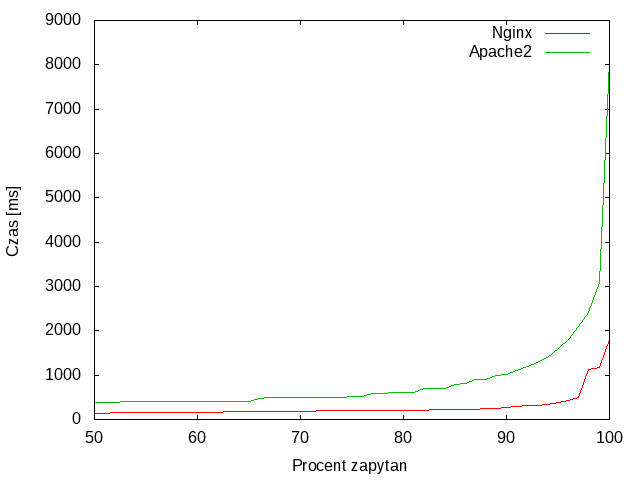
\includegraphics[width=\textwidth]{testy/wybor_index_duzy_128.png}
		\caption{128 równoległe zapytania}
	\end{subfigure}
	\begin{subfigure}[h]{0.3\textwidth}
		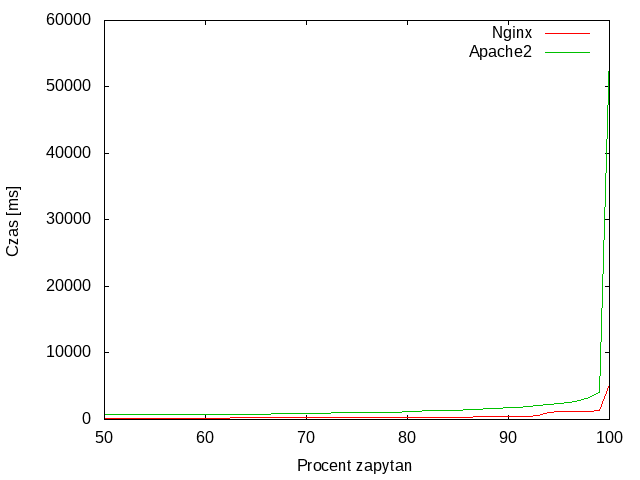
\includegraphics[width=\textwidth]{testy/wybor_index_duzy_256.png}
		\caption{256 równoległych zapytań}
	\end{subfigure}
	\caption{Zapytania o duży plik statyczny}\label{fig:wyb_index_duzy}
\end{figure}
Wykresy na rys.~\ref{fig:wyb_index_maly} przedstawiają czasy obsłużenia zapytań o plik HTML o rozmiarze 10 bajtów, natomiast wykresy na rys.~\ref{fig:wyb_index_duzy} czasy zapytań o plik o rozmiarze 100 kilobajtów.\\
Można zauważyć, że wyniki dla małych plików statycznych są zbliżone zarówno dla Apache jak i Nginx z lekką przewagą dla Nginx.
Największą przewagę Nginx-a widać przy średnim i dużym obciążeniu.
\clearpage
\subsection{Treść dynamiczna}
Testy treści dynamicznej przeprowadzane są przy użyciu konfiguracji Nginx + php-fpm oraz Apache + php-fpm.
Konfiguracja Apache + mod\_php została odrzucona, ponieważ wymaga umieszczenia serwera WWW oraz serwera PHP na jednym serwerze, co uniemożliwia użycie wielu serwerów PHP dla jednego serwera WWW.\\
Do testów zostały wykorzystane dwa bliźniacze skrypty obliczające liczby ciągu Fibonacciego.
Jeden ze skryptów został przedstawiony na listingu~\ref{lst:fib}.
Obliczane są wyrazy: piąty --- dla skryptu wykonującego się szybko, oraz piętnasty --- dla skryptu wykonującego się dłużej.\\
Wykorzystany został model obliczanie wartości rekurencyjny, ponieważ w przeciwieństwie do iteracyjnego wymaga większej mocy obliczeniowej.
Jest to pożądane aby czas obsługi zapytania obejmował czas wykonywania skryptu, a nie jedynie obsługi sesji HTTP oraz transferu danych (zostało to przetestowane przy wykorzystaniu \textit{szybkiego skryptu}).
\lstinputlisting[caption=fib.php,label=lst:fib,language=php]{lst/fib.php}
\begin{figure}
	\centering
	\begin{subfigure}[h]{0.3\textwidth}
		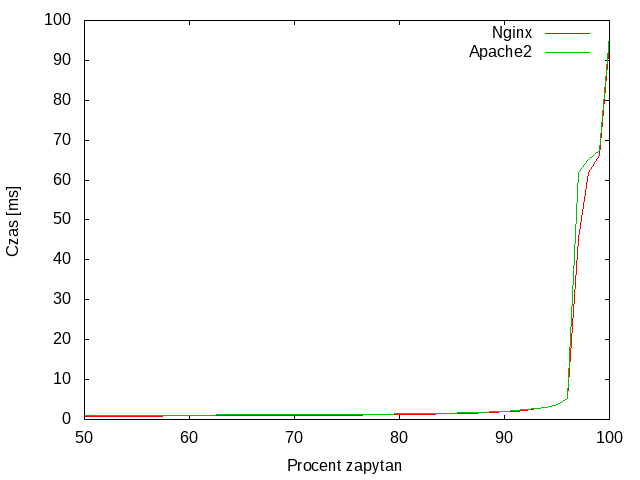
\includegraphics[width=\textwidth]{testy/wybor_fib_5_1.png}
		\caption{1 równoległe zapytanie}
	\end{subfigure}
	\begin{subfigure}[h]{0.3\textwidth}
		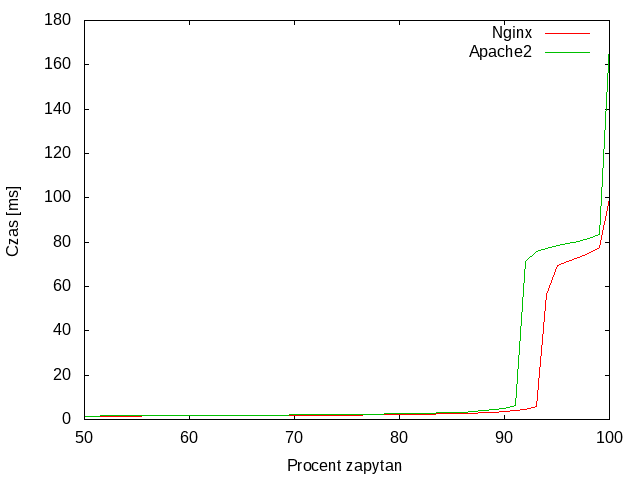
\includegraphics[width=\textwidth]{testy/wybor_fib_5_2.png}
		\caption{2 równoległe zapytania}
	\end{subfigure}
	\begin{subfigure}[h]{0.3\textwidth}
		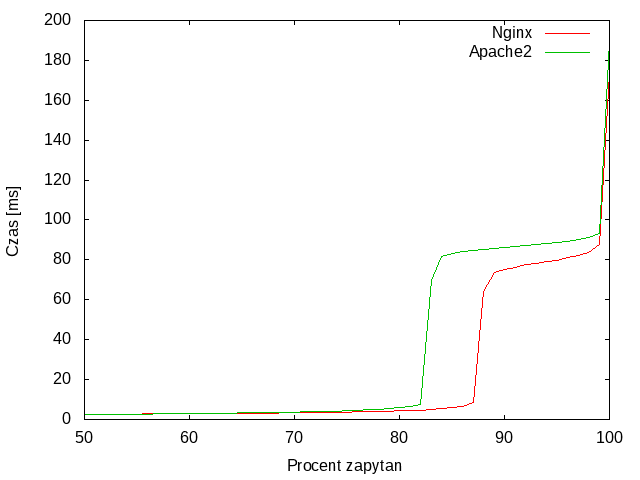
\includegraphics[width=\textwidth]{testy/wybor_fib_5_4.png}
		\caption{4 równoległe zapytania}
	\end{subfigure}

	\begin{subfigure}[h]{0.3\textwidth}
		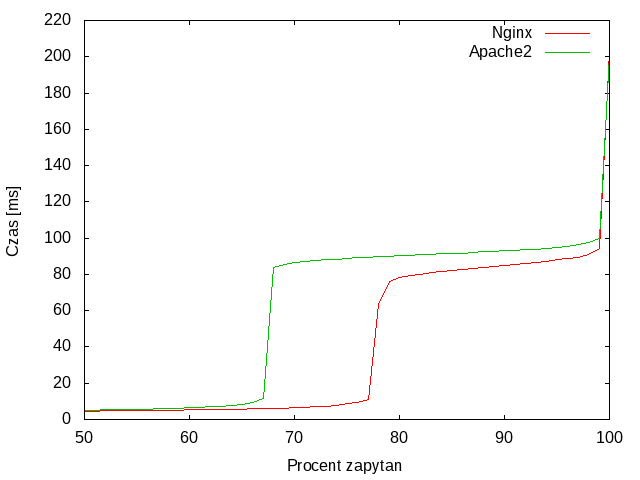
\includegraphics[width=\textwidth]{testy/wybor_fib_5_8.png}
		\caption{8 równoległych zapytań}
	\end{subfigure}
	\begin{subfigure}[h]{0.3\textwidth}
		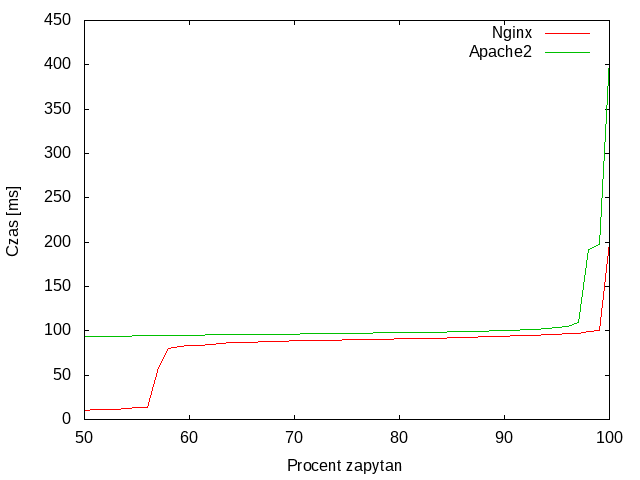
\includegraphics[width=\textwidth]{testy/wybor_fib_5_16.png}
		\caption{16 równoległych zapytań}
	\end{subfigure}
	\begin{subfigure}[h]{0.3\textwidth}
		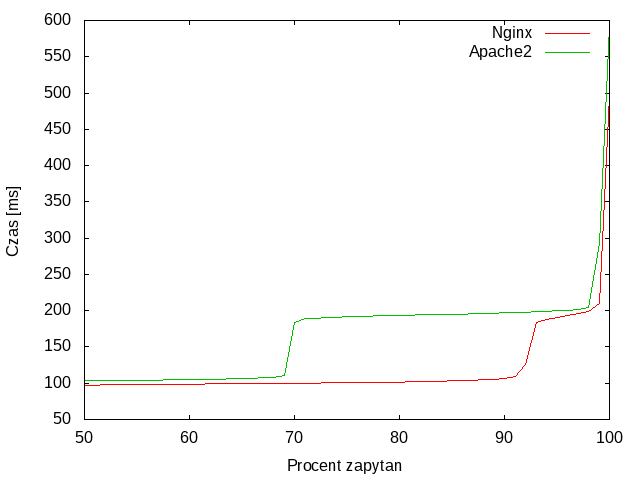
\includegraphics[width=\textwidth]{testy/wybor_fib_5_32.png}
		\caption{32 równoległe zapytania}
	\end{subfigure}

	\begin{subfigure}[h]{0.3\textwidth}
		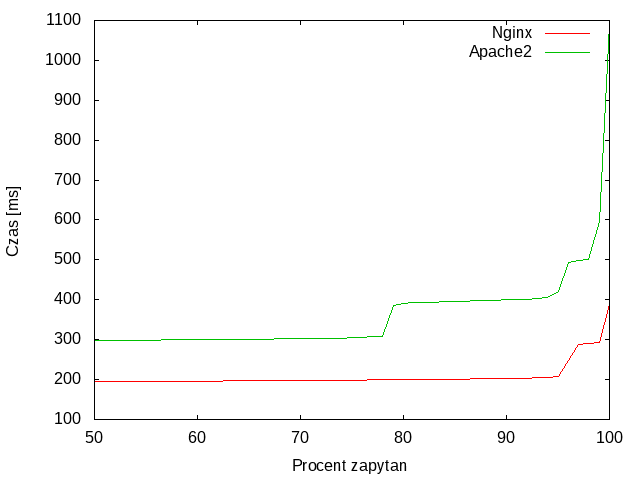
\includegraphics[width=\textwidth]{testy/wybor_fib_5_64.png}
		\caption{64 równoległe zapytania}
	\end{subfigure}
	\begin{subfigure}[h]{0.3\textwidth}
		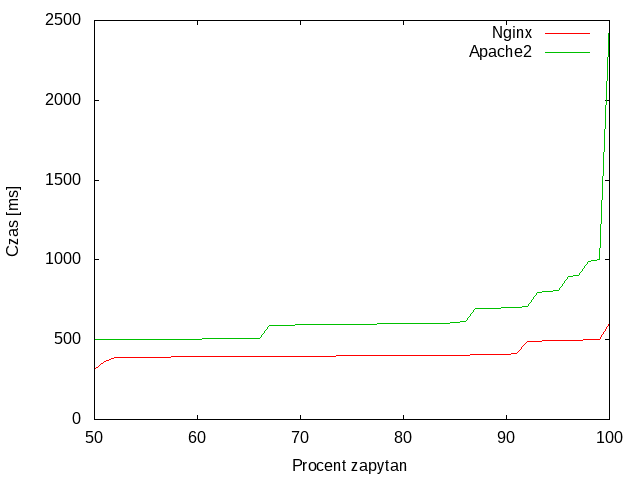
\includegraphics[width=\textwidth]{testy/wybor_fib_5_128.png}
		\caption{128 równoległe zapytania}
	\end{subfigure}
	\begin{subfigure}[h]{0.3\textwidth}
		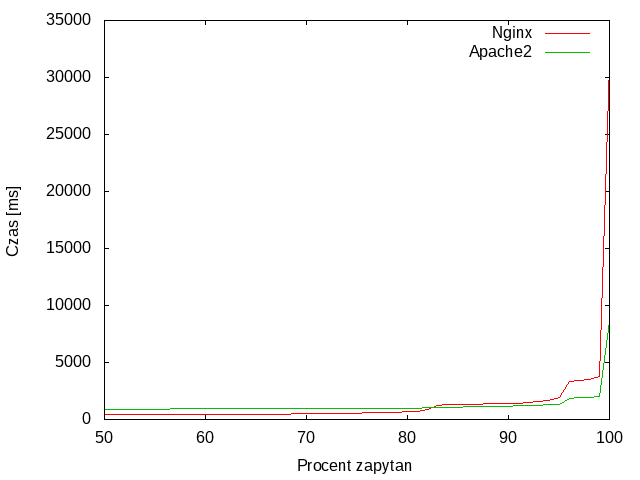
\includegraphics[width=\textwidth]{testy/wybor_fib_5_256.png}
		\caption{256 równoległych zapytań}
	\end{subfigure}
	\caption{Zapytania o szybki skrypt PHP}\label{fig:wyb_fib_5}
\end{figure}
\begin{figure}
	\centering
	\begin{subfigure}[h]{0.3\textwidth}
		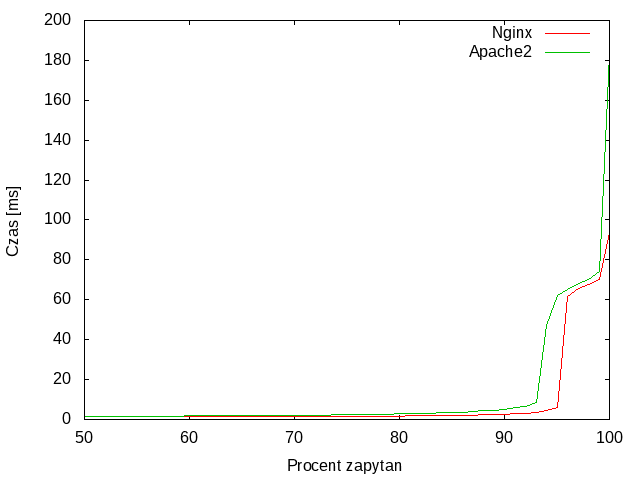
\includegraphics[width=\textwidth]{testy/wybor_fib_15_1.png}
		\caption{1 równoległe zapytanie}
	\end{subfigure}
	\begin{subfigure}[h]{0.3\textwidth}
		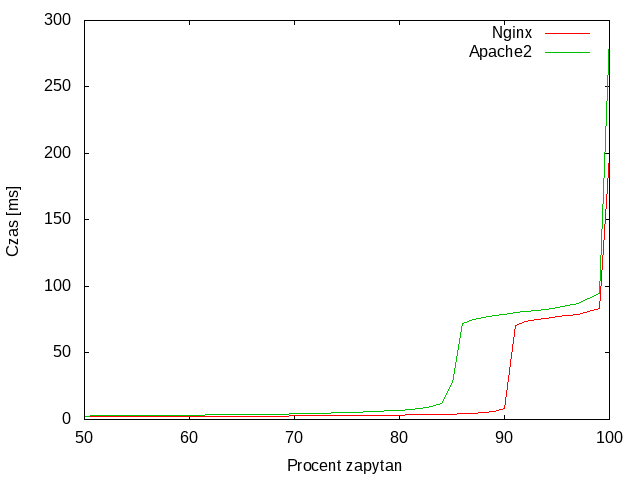
\includegraphics[width=\textwidth]{testy/wybor_fib_15_2.png}
		\caption{2 równoległe zapytania}
	\end{subfigure}
	\begin{subfigure}[h]{0.3\textwidth}
		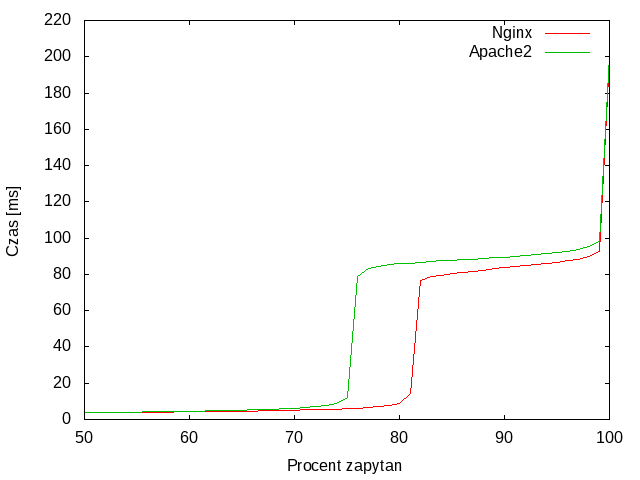
\includegraphics[width=\textwidth]{testy/wybor_fib_15_4.png}
		\caption{4 równoległe zapytania}
	\end{subfigure}

	\begin{subfigure}[h]{0.3\textwidth}
		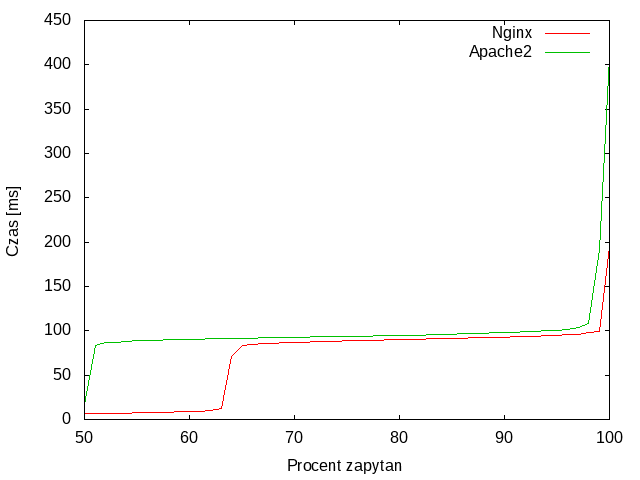
\includegraphics[width=\textwidth]{testy/wybor_fib_15_8.png}
		\caption{8 równoległych zapytań}
	\end{subfigure}
	\begin{subfigure}[h]{0.3\textwidth}
		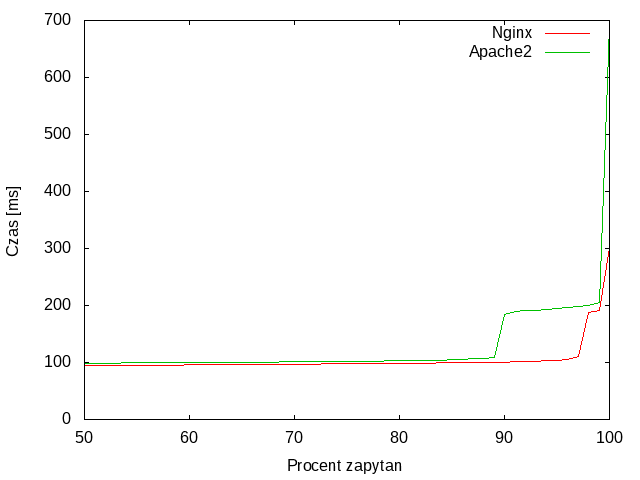
\includegraphics[width=\textwidth]{testy/wybor_fib_15_16.png}
		\caption{16 równoległych zapytań}
	\end{subfigure}
	\begin{subfigure}[h]{0.3\textwidth}
		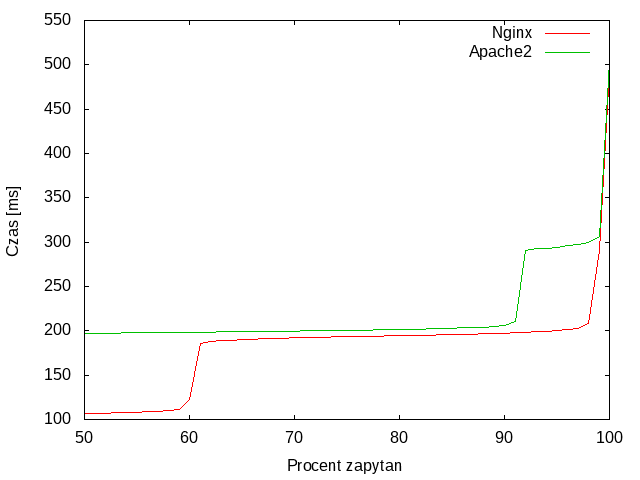
\includegraphics[width=\textwidth]{testy/wybor_fib_15_32.png}
		\caption{32 równoległe zapytania}
	\end{subfigure}

	\begin{subfigure}[h]{0.3\textwidth}
		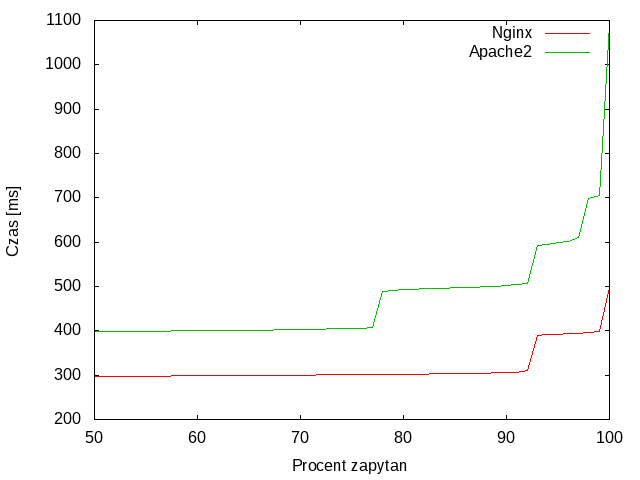
\includegraphics[width=\textwidth]{testy/wybor_fib_15_64.png}
		\caption{64 równoległe zapytania}
	\end{subfigure}
	\begin{subfigure}[h]{0.3\textwidth}
		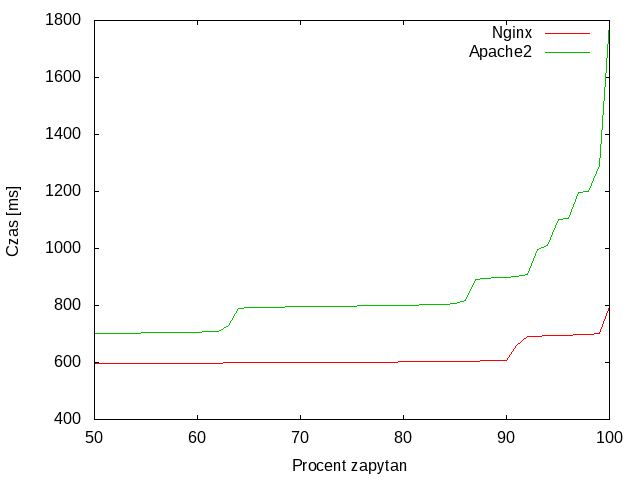
\includegraphics[width=\textwidth]{testy/wybor_fib_15_128.png}
		\caption{128 równoległe zapytania}
	\end{subfigure}
	\begin{subfigure}[h]{0.3\textwidth}
		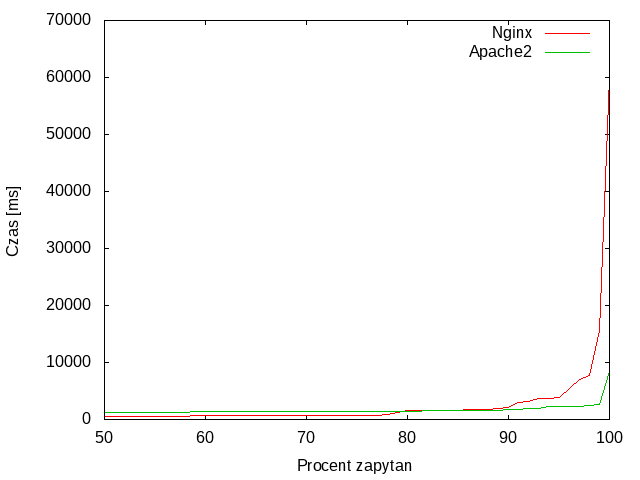
\includegraphics[width=\textwidth]{testy/wybor_fib_15_256.png}
		\caption{256 równoległych zapytań}
	\end{subfigure}
	\caption{Zapytania o wolny skrypt PHP}\label{fig:wyb_fib_15}
\end{figure}
Na wykresach~\ref{fig:wyb_fib_5} oraz~\ref{fig:wyb_fib_15} obrazujących czasy obsługi zapytań do skryptów PHP, można zauważyć że różnice pomiędzy Apache a Nginx są mniejsze niż dla plików statycznych.
Wynika to z faktu, ze obsługą zapytań w obu przypadkach zajmuje się PHP-fpm, natomiast serwer WWW odpowiedzialny jest jedynie za przekazywanie zapytań do \textit{backendu}.
\subsection{Podsumowanie}
Jak wykazały testy, Nginx daje krótsze czasy odpowiedzi we wszystkich testowanych sytuacjach, dlatego został wybrany jako podstawowy serwer wykorzystywany w przedstawionym projekcie.
\clearpage
\section{DNS round robin}
\subsection{Uwagi wstępne}
Jak zostało wspomniane w rozdziale~\ref{sec:dns}, DNS round robin nie jest metodą \textit{load balancingu} a jedynie wstępną metodą dystrybucji ruchu.
Pociąga to za sobą pewne konsekwencje.
Przeciętna aplikacja sieciowa, np: Chrome bądź links, dokonuje rozwiązania nazwy przy pierwszym odwołaniu się do danego adresu a następnie w celu zwiększenia wydajności, \textit{cachuje} jej adres.
Efektem tego takiego zachowania jest nawiązywanie późniejszych połączeń do tego samego adresu IP\@.
Aplikacja \textit{Apache Benchmark} która jest wykorzystywana do testowania rozwiązań w poniższej pracy również dokonywała jednorazowego rozwiązania nazwy i łączenia się do jednego adresu, co uniemożliwiało przeprowadzenie testów wydajnościowych \textit{DNS round robin} przy użyciu tego narzędzia.
Została zgłoszona poprawka\cite{ab_dnsrr} poprawiająca tą niedogodność.
Testy z wykorzystaniem tej poprawki symulują łączenie się dużej liczby niezależnych użytkowników.

Przy testowanie \textit{DNS round robin} nie zostanie przeprowadzona tak dokładna analiza jak przy wyborze serwera WWW, ponieważ metoda ta nie wpływa na działanie serwera WWW a jedynie na dystrybucję ruchu.

W testach tych, w przeciwieństwie do wyboru serwera WWW, użyto opcji \texttt{Keep Alive} powodującej utrzymywanie połączenia i wykonywanie kolejnych bez ponownego nawiązywania połączeń TCP\@.
W przypadku użycia poprawki~\cite{ab_dnsrr} każde połączenie jest tworzone do serwera wynikającego z technologi \textit{DNS round robin} a następnie jest ono utrzymywane aż do zakończenia programu. Liczba połączeń zależy od parametru \texttt{concurrent}
\subsection{Testy wydajnościowe}
Testowanie rozwiązania \textit{DNS round robin} zostanie przedstawione na odpytywaniu jedynie pliku statycznego ponieważ testy dla pozostałych treści będą analogiczne do tych przedstawionych w rozdziale~\ref{sec:wybor}.\\
Do testów został wykorzystany \textit{DNS round robin} przedstawiony na listingu~\ref{lst:test_dnsrr}.
\lstinputlisting[caption=DNS round robin, label=lst:test_dnsrr]{lst/test_dnsrr.bash}
Zawiera on cztery serwery z identyczną konfiguracją.\\
Wykresy~\ref{fig:test_dnsrr} przedstawiają czasy obsługi zapytań w przypadku pojedynczego serwera WWW oraz grupy serwerów z dystrybucją ruchu poprzez \textit{DNS round robin}.
Na wykresach został pominięty czas najdłuższego połączenia z powodu małego wkładu informacyjnego oraz dużego stopnia zaciemniania obrazu.
\wykresy{dnsrr}{Dystrybuja ruchu w oparciu o DNS RR}{test_dnsrr}
Tabela~\ref{tab:test_dnsrr} przedstawia liczbę obsłużonych zapytań na sekundę.
\begin{table}[h]
\centering
\begin{tabular}{cccc}
	\toprule
	Liczba połączeń & Nginx & DNS RR & Przyrost\\
	\midrule
	\midrule
	1&2571&4301& +67\%\\
	\midrule
	2&2001&5458& +172\%\\
	\midrule
	4&1353&6264& +362\%\\
	\midrule
	8&1704&7582& +344\%\\
	\midrule
	16&2097&8720& +315\%\\
	\midrule
	32&2133&7484& +250\%\\
	\midrule
	64&1968&10617& +439\%\\
	\midrule
	128&1945&10194& +424\%\\
	\midrule
	256&2190&9821& +348\%\\
	\bottomrule
\end{tabular}
\caption{Obsłużonych zapytań na sekundę}
\label{tab:test_dnsrr}
\end{table}
\subsection{Podsumowanie}
Jak można zaobserwować na wykresach, użycie dystrybucji ruchy zmniejsza czasy oczekiwania na przetworzenie zapytań.\\
Dane przedstawione w tabeli~\ref{tab:test_dnsrr} pokazują, iż użycie czterech serwerów zamiast jednego daje w większości przypadków przyrost ok 300\%, co jest wartością oczekiwaną, ponieważ przy użyciu trzech dodatkowych serwerów oczekujemy trzykrotnego przyrostu wydajności.\\
W przypadku jednego równoległego połączenia oczekiwanym przyrostem były przyrost 0\% ponieważ wykonywane jest jedno połączenie, jednak specyfika serwera Nginx jest taka, że po przyjęciu stu połączeń w trybie \texttt{Keep-Alive} zamyka on połączenie.
Następuje wtedy nawiązanie kolejnego, które zostaje przekierowane do kolejnego serwera z puli \textit{DNS round robin}.
Jest to przyczyną zwiększonego przyrostu dla jednego i dwóch równoległych połączeń.\\
Przy liczbie połączeń cztery i więcej powyższy efekt nie ma znaczenia, ponieważ w obsłudze zapytań biorą udział wszystkie serwery.
\section{LVS}
W tej sekcji przetestowany zostanie LVS w trybie \textit{direct routing}, ponieważ jest on najrozsądniejszym trybem.
Testom poddany zostanie narzut wynikający z użycia LVS, jak również przetestowane zostaną rozwiązanie bliższe rzeczywistości, czyli zawierające kilka \textit{real server}-ów.
Ponadto, sprawdzone zostanie zachowanie LVS w warunkach nieidealnych, tj.\ w przypadku awarii jednego z \textit{real server}-ów oraz w przypadku wysycenia łącza.
\subsection{Uwagi dotyczące urządzeń sieciowych}
\label{sub:uwagi_sieciowe}
Ponieważ w omawianym rozwiązaniu występuje jeden węzeł do którego nawiązywane są połączenia, parametry łącza są w tym przypadku (w przeciwieństwie do DNS round robin gdzie klient łączy się do różnych serwerów) istotne.
\begin{description}
	\item{Maszyna z \textit{directorem}}
		\begin{itemize}
			\item Wirtualizowany sterownik karty sieciowej: rtl8139
			\item Szybkość karty podawana przez ethtool: 100Mb/s
		\end{itemize}
	\item{Maszyna z LXC}
		\begin{itemize}
			\item Wirtualizowany sterownik karty sieciowej: virtio
			\item Szybkość karty podawana przez ethtool: Brak
		\end{itemize}
	\item{Maszyna z Nginx}
		\begin{itemize}
			\item Wirtualizowany sterownik karty sieciowej: wirtualny interface hosta
			\item Szybkość karty podawana przez ethtool: 10000Mb/s
		\end{itemize}
\end{description}
Na uwagę zasługują tutaj parametry maszyny będącej hostem dla LXC\@.
Użycie sterownika \texttt{virtio} pozwala maszynie wirtualizowanej komunikować się z maszyną hostującą bez emulacji konkretnych sterowników sieciowych, lecz już na poziomie jądra.
Dlatego nie jest możliwe określenie prędkości takiego interface-u, ponieważ zasada jego działania jest inna niż rzeczywistych kart sieciowych.\\
Podobnie sytuacja wygląda dla kontenerów LXC\@.
Tam komunikacja następuje poprzez wirtualne interface-y na jeden maszynie, dlatego prędkość podana przez \texttt{ethtool} wynosi 10Gb/s.

W przypadku testowania zachowania rozwiązania na wysycenie łącza, zastosowany zostanie duży plik HTML o rozmiarze ok 1MB.
Pozwoli to zasymulować sytuacje w której żądany ruch będzie większy niż możliwości łącza serwera.
\subsection{Narzut własny LVS}
\label{sec:lvs_narzut}
Aby sprawdzić jakie opóźnienie generuje mechanizm LVS, skonfigurowany zostanie jeden serwer \textit{director} oraz jeden \textit{real server}.
Porównując czasy odpowiedzi serwera WWW odpytywanego bezpośrednio oraz poprzez LVS, otrzymamy jaki wpływ na działanie ma LVS\@.
Żądany będzie mały plik statyczny.
\wykresy{one_lvs_maly}{Narzut własny LVS}{one_lvs_maly}

Jak widać na rysunku~\ref{fig:one_lvs_maly}, czasy odpowiedzi serwera bezpośrednio oraz poprzez LVS nie odbiegają zbytnio od siebie.
Różnica na wykresie jest widoczna jedynie dla jednego konkurencyjnego zapytania, jednak wartość tych czasów (0.2ms i 0.4ms) są na tyle małe, ze ta różnica może zostać pominięta.
\subsection{Wiele real serverów}
Rozważmy teraz przypadek, w którym mamy cztery takie same serwery WWW\@.
Zostały skonfigurowane 3 usługi LVS\@. Tą konfiguracje przedstawia listing~\ref{lst:four_lvs_maly}.
\footnotesize
\lstinputlisting[caption=LVS z wieloma serwerami,label=lst:four_lvs_maly]{lst/four_lvs_maly}
\normalsize
Widzimy, ze każda z usług posiada inną liczę serwerów oraz posiada taki sam algorytm balansowania.
Każdy z serwerów ma wagę 1 oraz każdy jest wykorzystywany w trybie \textit{direct routing}.

\wykresy{four_lvs_maly}{Czasy odpowiedzi LVS w zależności od ilości serverów}{four_lvs_maly}
Wykresy~\ref{fig:four_lvs_maly} przedstawiają czasy odpowiedzi w zależności o ilości \textit{real server}-ów.
Wymaga on trochę dokładniejszej analizy niż poprzednie wykresy.
Dla jednego równoległego zapytania, widzimy ze czasy każdej z usług LVS są gorsze niż bezpośrednie zapytania do server WWW\@.
Dzieje się tak dlatego, ze mając jedno równoczesne zapytanie, wykorzystywany jest tylko jeden serwer na raz, czyli jest to sytuacja tożsama z rozdziałem~\ref{sec:lvs_narzut}.\\
W przypadku 2 połączeń, wykresy zaczynają się zbiegać, ponieważ narzut LVS zaczyna być kompensowany poprzez dystrybucję zapytań.\\
Począwszy od czterech zapytań, zauważamy że połączenia kierowane do LVS są obsługiwane szybciej.
Najbardziej jest to widoczne przy dużym obciążeniu serwera, tj. 128 i 256 równoległych zapytań.
\subsection{Odporność na błędy}
W rozdziale tym, omówione zostanie obsługiwanie błędów przez LVS.
\subsubsection*{Obsługa wysokiej wydajności}
Niestety narzędzie wykorzystywane w tej pracy do testowania wydajności rozwiązań, posiada bardzo ubogą obsługę błędów, dlatego nie zostaną zamieszczone żadne wykresy.\\
Ponieważ LVS jest narzędziem nastawionym na wydajność i mały rozmiar, nie wspiera natywnie sprawdzania dostępności usług na \textit{real server}-ach.
W przypadku niedostępności usługi, pakiet zostaje przekazany do \textit{real server}-a, który natomiast odpowiada błędem.
Mogą to być błędy \texttt{connection refused, timeout, file not found} bądź wiele innych.
Taki też błąd zostaje przekazany do klienta.\\
Sytuacja taka wynika z kilku czynników.
Jednym z nich jest tryb działania LVS:
\begin{description}
	\item{LVS DR/TUN}\\
		W tym trybie odpowiedź jest kierowana bezpośrednio do klienta.
		W związku z tym, \textit{director} nie jest świadomy błędnej odpowiedzi \textit{real server}-a, dlatego nie może ponowić zapytania do innego, działającego.
	\item{LVS NAT}\\
		W tym przypadku, ruch powracający przechodzi ponownie przez \textit{directora} i istnieje techniczna możliwość wykrywania błędów w odpowiedzi.
		Jednak, aby zachować homogeniczność zachowania w każdym trybie, nie jest to wykonywane.
\end{description}
Kolejną przyczyną takiego zachowania LVS jest warstwa w której on pracuje.
Jego głównym zadaniem jest przekazywanie pakietów i ingerencja w nie jedynie na warstwie drugiej a inspekcja jedynie do warstwy czwartej.
Tak niskie działanie usługi w znacznym stopniu ograniczyło by możliwości monitorowania usług na \textit{real server}-ach do sprawdzania możliwości połączenia na dany port (co w wielu przypadkach wystarcza).\\
Ponadto, LVS nastawiony jest na wydajność i dążenie, aby jego kod był jak najmniejszy i najszybszy.
Dodanie do niego kodu obsługującego różne scenariusze sprawdzania dostępności usługi obniżyłyby tą wydajność.

Wszystkie powyższe powody sprawiają, że aby dodać do LVS wsparcie dla wysokiej dostępności, należy użyć dodatkowych narzędzi.
Bądź po stronie LVS, które sprawdzają dostępność usług (na dowolnym poziomie) i ewentualnie \textit{wypinają} z LVS niedostępne serwery, bądź rzadziej, po stronie \textit{real server}-ów zastosowanie \texttt{floating IP}, nadające innej, działającej maszynie adres IP maszyny która uległa awarii.
\subsubsection*{Zachowanie w przypadku awarii}
Jak zostało wspomniane w poprzednim paragrafie, \textit{real server} odpowiada bezpośrednio do klienta, dlatego w przypadku awarii jednego z serwerów, zapytania kierowane na niego zostaną odrzucone.
Spowoduje to zwrócenie błędu do klienta. Ten może to odczuć na kilka sposobów, np w przypadku stron WWW, jeżeli zapytanie o plik \texttt{index.html} zostanie przekazane do niedziałającego serwera, klient otrzyma w przeglądarce informację \texttt{connection refused}.
Po odświeżeniu strony, zapytanie powinno trafić na inną maszynę, która zwróci treść strony.\\
To prowadzi do kolejnej sytuacji, w której zapytanie o \texttt{index.html} zakończyło się sukcesem, natomiast zapytania o kolejne pliki statyczne będą trafiać na niedziałającą maszynę.
Spowoduje to niewczytanie się obrazów, arkuszy stylów bądź skryptów \texttt{java script}.
Jest to sytuacja bardziej irytująca dla użytkownika, ponieważ zostaje mu przedstawiona część treści na stronie, lecz zwykle w sposób niepozwalający na jej komfortowe przeglądanie.\\
Trzecią sytuacją która może wystąpić - będącą chyba najgroźniejszą pod kątem logistycznym - jest poprawne załadowanie się całej treści strony, jednak zapytania dynamicznie generowane przez np: \texttt{Ajax}-a trafiają na niedziałający serwer i nie są przetwarzane.
Zwykle klient nie jest informowany o niepowodzeniu przy takim zapytaniu, bądź jest informowany o niepowodzeniu bez podawania przyczyny.
Jest to szczególnie niebezpieczne przy wykonywaniu ważnych operacji typu składanie wniosków bądź robienie przelewów w banku.
\subsubsection*{Wysycenie łącza}
\label{sub:lvs_wysycenie_lacza}
Do testowanie wysycenia łącza, został wybrany plik o rozmiarze 1MB.
Niestety przy badanych maszynach nie udało się osiągnąć pełniej mocy łącza, a jedynie ruch na poziomie 900KB/s.
Sytuacja taka spowodowana jest utylizacją pracy procesora na poziomie 95\%.\\
Tak wysokie zużycie CPU wynika z potrzeby przekazania wszystkich pakietów \texttt{ACK} wracających od klienta.

Powyższy test pokazuje, iż LVS jest odporny na problem wysycenia łącza i jego wydajność ograniczają inne parametry maszyny.\\
W przeprowadzanym teście, przybliżona wartość wydajności wynosi ok 320 zapytań na sekundę.
\subsection{Podsumowanie}
Wykonane testy pokazują, iż \textit{Linux Virtual Server} jest technologią bardzo wydajną.
Jej narzut własny jest bliski zeru, natomiast przy większej ilości serwerów następuje bardzo efektywny rozdział zapytań.\\
Niestety LVS nie posiada żadnych metod wykrywania awarii \textit{real server}-ów, dlatego w tym celu należy użyć dodatkowych narzędzi.
\begin{table}[h]
\centering
\begin{tabular}{cccc}
	\toprule
	Liczba połączeń & Nginx & LVS 4xRS & Przyrost\\
	\midrule
	\midrule
	1&2697.30&2722.17&0\%\\
	\midrule
	2&2148.13&4610.76&114\%\\
	\midrule
	4&2182.04&5619.42&157\%\\
	\midrule
	8&1934.86&8103.03&318\%\\
	\midrule
	16&2182.62&8940.06&309\%\\
	\midrule
	32&2333.41&10542.87&351\%\\
	\midrule
	64&2278.52&9411.09&313\%\\
	\midrule
	128&2390.89&10907.20&356\%\\
	\midrule
	256&2648.01&9499.84&258\%\\
	\bottomrule
\end{tabular}
\caption{Obsłużonych zapytań na sekundę}
\label{tab:test_lvs}
\end{table}
Tabela~\ref{tab:test_lvs} potwierdza przedstawione wnioski.
W przypadku jednego połączenia przyrost wynosi 0, natomiast dla połączeń 8 i więcej, przyrost oscyluje około wartości 300, co jest wartością oczekiwaną.
\section{Haproxy}
Rozdział ten skupi się na przetestowaniu wydajności aplikacji Haproxy, oraz jej odporności na awarie serwerów \textit{backend}-owych.
\subsection{Uwagi dotyczące urządzeń sieciowych}
W celu zachowania porównywalnego środowiska co LVS, zostaną zastosowane wytyczne z rozdziału~\ref{sub:uwagi_sieciowe}.
\subsubsection{Wydajność}
Rozdział ten skupi się na przetestowaniu wydajności Haproxy.
Testowane zostanie bezpośrednie połączenie do Nginx-a oraz połączenia czterech usług Haproxy, zawierające odpowiednia, jeden, dwa, trzy i cztery serwery \textit{backend}-owe.\\
Zapytania, podobnie jak w LVS będą kierowane o mały plik statyczny.
\wykresy{four_haproxy_maly}{Czasy odpowiedzi Haproxy w zależności od ilości serwerów}{four_haproxy_maly}
Wykres~\ref{fig:fout_haproxy_maly} przedstawia czasy odpowiedzi Haproxy oraz Nginxa w zależności od ilości równoległych zapytań.\\
Jak można zauważyć, dla niewielkiej liczby równoległych zapytać, czasy odpowiedzi Haproxy są zbliżone do natywnego Nginx-a.
Wzrost wydajności widać dopiero przy większej ilości zapytań, tj. od około 64 równoległych zapytań.
\subsection{Odporność na awarie}
\subsubsection{Awaria serwerów \textit{backendowych}}
Ponieważ Haproxy został zaprojektowany z myślą o wysokiej dostępności, posiada on natywną obsługę wykrywania awarii serwerów.
W przypadku wykrycia awarii, dany serwer zostaje oznaczony jako \texttt{DOWN} i nie zostają do niego przekazywane zapytania.
Zmniejsza to wydajność całego klastra, jednak zapytania użytkownika zostają przekazane do działających maszyn, dzięki czemu, klient zawsze otrzymuje odpowiedź.\\
Aby zobrazować zachowanie Haproxy na awarie maszyn, zostaną przeprowadzone testy wydajnościowe z wszystkimi czterema serwerami działającymi, a następnie te same testy zostaną powtórzone dla wyłączonych usług Nginx na jednym, dwóch oraz na trzech maszynach.\\
Testy dla wyłączonych czterech maszyn nie zostaną przeprowadzone, ponieważ z powodu braku jakiekolwiek serwera \textit{backend}-owego, klient nigdy nie otrzyma odpowiedzi.
\wykresy{haproxy_awaria_wezlow}{Czasy odpowiedzi Haproxy w zależności od ilości serwerów i awarii węzłów}{haproxy_awaria_wezlow}
Wykresy przedstawione na rysunku~\ref{fig:haproxy_awaria_wezlow} pokazują, że awaria węzłów nie powoduje błędnych odpowiedzi do klienta.
Poprzednie spostrzeżenie jest prawdziwe pomijając drobną anomalię dla 32 i 64 połączeń, gdzie Haproxy z trzeba niedziałającymi serwerami daje trochę gorsze odpowiedzi.

Powyższe testy zapytań były przeprowadzane dopiero po ustaleniu przez Haproxy, niedostępności usługi po jej wyłączeniu.
\subsubsection*{Awaria węzła w trakcie obsługi zapytań}
Poprzedni rozdział wykazał, iż po ustaleniu się stanu \texttt{DOWN} dla serwerów \textit{backend}-owych, Haproxy nie powoduje żadnych błędów w odpowiedziach do klienta.\\
Kolejnym testem dla wysokiej dostępności jest zachowanie się Haproxy w przypadku awarii serwera dla połączeń obsługiwanych po awarii serwera a przed wykryciem tego faktu przez system.\\
Haproxy sprawdza dostępność usługi co jedną sekundę, natomiast po trzeciej nieudanej próbie połączenia, uznaje usługę za niedostępną.
W efekcie, powstaje trzy sekundowe \textit{okno} w którym klient może uzyskać odpowiedź o niedostępności usługi.\\
Test polegał na ciągłym wysyłaniu 128 równoległych zapytań do serwera.
W tym samym czasie nastąpiło wyłączenie usługi Nginx na jednym z serwerów.
W trakcie trzy sekundowego \textit{okienka}, zostało zwróconych od 50 do 150 błędów (w zależności od uruchomienia testu).\\
Cały test trwał 14 sekund. W jego trakcie zostało wykonanych 30000 zapytań z czego ok 100 zakończyło się niepowodzeniem.
W mojej opinii jest to bardzo wysoki poziom dostępności usługi.
\subsubsection*{Wysycenie łącza}
Warunki testowanie wysycenia łącza dla Haproxy są analogiczne do tych stosowanych w LVS (rozdział~\ref{sub:lvs_wysycenie_lacza}).\\
W tym przypadku procesor podobnie został obciążony na 100\%.
Wykorzystanie łącza utrzymywało się na poziomie 10MB/s, natomiast liczba obłużonych zapytań na sekundę wynosiła około 20.
\subsection{Podsumowanie}
Jak wykazały testy, Haproxy daje bardzo duży poziom wysokiej dostępności.
Można zauważyć bardzo krótki czas wykrywania niedostępności usługi, oraz bardzo dobrą reakcje minimalizującą ilość błędów zwracanych do klienta.\\
\begin{table}[h]
  \centering
  \begin{tabular}{cccc}
      \toprule
      Liczba połączeń & Nginx & Haproxy 4xRS & Przyrost\\
      \midrule
      \midrule
	  1&2741.46&1521.45&-44\%\\
      \midrule
	  2&2142.82&2207.01&2\%\\
      \midrule
	  4&2006.00&2940.17&46\%\\
      \midrule
	  8&2133.27&3563.32&67\%\\
      \midrule
	  16&2139.60&3532.11&65\%\\
      \midrule
	  32&2226.88&4067.57&82\%\\
      \midrule
	  64&2335.50&3930.86&68\%\\
      \midrule
	  128&2183.21&4189.07&91\%\\
      \midrule
	  256&2394.04&2875.26&20\%\\
      \bottomrule
  \end{tabular}
  \caption{Przyrost obsłużonych zapytań przez Haproxy}
  \label{tab:test_haproxy}
  \end{table}
Tabela~\ref{tab:test_haproxy} przedstawia przyrost wydajności względem pojedynczego serwera WWW~.
Można zauważyć, że dla jednego połączenia mamy przyrost ujemny.
Wartości przyrostów dla większej liczby połączeń również nie są zbyt wysokie.
Sytuacja ta wynika z faktu zapotrzebowania na dużą moc obliczeniową związaną z \textit{Nat}-owaniem pakietów oraz przeliczaniem adresów.
\section{Porównanie LVS oraz Haproxy}
Jak wykazały testy, oba omawiane systemy służą do balansowania połączeń pomiędzy realne serwery obsługujące zapytania.
Zadaniem administratora jest ocena i wybór odpowiedniego narzędzia do odpowiedniej sytuacji.\\
Dla dużego ruchu odpowiedniejszy wydaje się LVS, gdyż jest dużo bardziej wydajny, jednak nie wspiera natywnie wysokiej dostępności.
Administrator jest odpowiedzialny za dobranie innego narzędzia dodającego obsługę awarii serwerów, aby klient nie otrzymywał błędnych komunikatów zwrotnych.\\
Natomiast przy obsłudze mniejszego ruchu, Haproxy zyskuje dzięki dobremu systemowi wykrywania awarii, co zapewnia ciągłą dostępność usługi dla klienta.

Warto zwrócić uwagę, ze dla jednego i dwóch równoległych połączeń, zarówno Haproxy jak i LVS mają bardzo dobre czasy odpowiedzi.
Różnice zaczynają się dopiero dla większego obciążenia, co zostało wyjaśnione w poprzednim paragrafie.

Dodatkowo, można zauważyć różnicę w wykorzystaniu łącza.
W testowanym środowisku, ani Haproxy ani LVS nie wysyciły łącza, gdyż procesor był elementem limitującym możliwości obu metod, jednak różnica wykorzystania łącza przy obecnych parametrach, pozwala wysnuć teorię, że przy wykorzystaniu mocniejszych maszyn w środowisku produkcyjnym, różnica ta może mieć znaczenie, gdy ich możliwości zaczną być limitowane przez łącze.
\section{Nietestowane rozwiązania}
W tym rozdziale nie zostały poruszone wszystkie kwestie związane z wysoką dostępnością.
Oto najważniejsze pozycje które nie zostały przetestowane.
\begin{itemize}
	\item możliwości Nginx-a do rozdzielania połączeń.
		Zostały pominięte ponieważ możliwość wykrywania niedostępności usług jest dostępna jedynie w płatnej subskrypcji. Z powodu mnogości darmowych rozwiązań open source-owych, płatne moduły nie były testowane.
	\item heartbeat/keepalied/ldirector/\ldots - szereg narzędzi dodających funkcjonalność wysokiej dostępności do LVS.
	\item corosync/\ldots - narzędzia do zapewniania wysokiej dostępności dla urządzeń brzegowych.\\
		Pozwalają ustawić tzw. \textit{floating IP}.
		W przypadku awarii jednej maszyny (np: \textit{director}-a LVS), druga, zapasowa, wykrywa ten fakt i ustawia odpowiednie adresy na swoim interface-ie oraz konfiguruje odpowiednie usługi, tak, aby móc przejąć funkcje maszyny która uległa awarii.
\end{itemize}
